\documentclass{Style/Boostan-ThesisR}

% تعیین عنوان پروژه
\title{
شبکه‌های اقتضایي و کاربردهای }
% نام نویسنده
\author{حسن احمدی}
% تعیین تاریخ ارایه پروژه 
\date{مهر ۱۳۹۲}
%% استاد راهنما
\supervisor{دکتر حسین محمدی}

\adviser{دکتر حسن ابراهیمی}

\institute{دانشگاه تهران}
\faculity{پردیس دانشکده فنی}
\group{دانشکده برق و کامپیوتر}

\comment{کارشناسی ارشد}

%\farsimajor{مهندسی کامپیوتر، گرایش هوش ماشین و رباتیک}

\englishtitle{Hello Hello Wireless Ad Hoc Network In Vehicular Ad Hoc Network And Today Application Is}

\englishAuthor{Hoessien Sys}

\englishsupervisor{Dr. Ali Ali De}

\englishadvisor{Dr. Ali Mohmmad Ehsan}

\englishDate{Aug 2012}



%%%%% Num

\newacronym{3GPP}{3GPP}{3rd Generation Partnership Projec}



%%%%% A
\newacronym{AAA}{AAA}{Authentication, Authorization and Accounting}

\newacronym{AB}{AB}{Access Burst}

\newacronym{ABMF}{ABMF}{Account Balance Management Function}

\newacronym{ACCH}{ACCH}{Associated Control Channel}


\newacronym{BSS}{BSS}{Base Station Subsystem}

\newacronym{BSSAP}{BSSAP}{Base Station Subsystem Application Part}

\newacronym{BSSLAP}{BSSLAP}{BSS Location Service Assistance Protocol}

\newacronym{BSSMAP}{BSSMAP}{BSS Management Application Part protocol}

\newacronym{BTS}{BTS}{Base transceiver station}

%%%%% C
\newacronym{CA}{CA}{Certificate authority}

\newacronym{CAN}{CAN}{Campus Area Network}

\newacronym{CAP}{CAP}{CAMEL Application Part}

\newacronym{CAMEL}{CAMEL}{Customised Applications for Mobile networks Enhanced Logic}

\newacronym{CBC}{CBC}{Cell Broadcast}

\newacronym{PSNR}{PSNR}{Peak Signal to Noise Ratio }



% حتما بین هر دو کلمه اختصاری که تعریف می کنید یک خط فاصله باشد.

% فاصله




%%%% A

\newglossaryentry{Absorption}
{name={Absorption}, 
plural={جذب},
description={}
}

\newglossaryentry{AcceptableCell}
{name={Acceptable Cell}, 
plural={سلول پذیرفتنی},
description={}
}

\newglossaryentry{Accessibility}
{name={Accessibility}, 
plural={دستیابی‌پذیری},
description={}
}

\newglossaryentry{AccessBurst}
{name={Access Burst}, 
plural={توده دسترسی},
description={}
}

\newglossaryentry{AccessPoint}
{name={Access Point}, 
plural={نقطه دسترسی},
description={}
}
\newglossaryentry{AccessDomain}
{name={Access Domain}, 
plural={ناحیه دسترسی},
description={}
}

\newglossaryentry{AccessStratum}
{name={Access Stratum}, 
plural={طبقه دسترسی},
description={}
}

\newglossaryentry{Accounting}
{name={Accounting}, 
plural={حسابرسی},
description={}
}

\newglossaryentry{AccountingManagement}
{name={Accounting Management}, 
plural={مدیریت حسابرسی},
description={}
}

\newglossaryentry{Accuracy}
{name={Accuracy}, 
plural={دقت},
description={}
}

\newglossaryentry{Achievable}
{name={Achievable}, 
plural={قابل دستیابی},
description={}
}

\newglossaryentry{Action}
{name={Action}, 
plural={کنش},
description={}
}

\newglossaryentry{Actions}
{name={Actions}, 
plural={کنش‌ها},
description={}
}

\newglossaryentry{ActiveState}
{name={Active State}, 
plural={حالت فعال},
description={}
}

\newglossaryentry{AdHocNetwork}
{name={AdHoc Network}, 
plural={شبکه اقتضایی},
description={}
}

\newglossaryentry{AdHocNetworks}
{name={AdHoc Networks}, 
plural={شبکه‌های اقتضایی},
description={}
}

\newglossaryentry{Adjacent}
{name={Adjacent}, 
plural={مجاور},
description={}
}

\newglossaryentry{AdjacentChannelInterference}
{name={Adjacent Channel Interference}, 
plural={تداخل کانال‌های همجوار},
description={}
}

\newglossaryentry{Adversary}
{name={Adversary}, 
plural={مهاجم},
description={}
}

\newglossaryentry{Aeronavigation}
{name={Aero Navigation}, 
plural={ناوبری هوایی},
description={}
}

\newglossaryentry{Aggregate}
{name={Aggregate}, 
plural={تجمیع شده},
description={}
}

\newglossaryentry{AggregateFunction}
{name={Aggregate Function}, 
plural={تابع تجمیع شده},
description={}
}

\newglossaryentry{AggregateProcess}
{name={Aggregate Process}, 
plural={فرایند تجمیع شده},
description={}
}

\newglossaryentry{AggregateThroughput}
{name={Aggregate Throughput}, 
plural={گذردهی تجمیع شده},
description={}
}

\newglossaryentry{Agreed}
{name={Agreed}, 
plural={موافقت شده},
description={}
}


\textwidthfootnoterule

\begin{document}



% صفحه بسم‌الله، فایل god در پوشه Pic قرار دارد. 
\Godpage{Pic/god}
% صفحه عنوان فارسی، با دو لوگو هر دو لوگو در پوشه Pic وجود دارد. 
\thesisStyleOO
% صفحه امضا
\clearpage\newpage
\thispagestyle{empty}
\begin{table}
\begin{tabular}{ccc}

\includegraphics[width=.15\textwidth]{Pic/logo}&
\begin{minipage}{0.55\linewidth}
\vskip 0.9cm
\begin{center}\Large
\typefontR{\Large
دانشگاه تهران 
}
 \\* [0.5cm]
پردیس دانشکده فنی\\ [0.5cm]
\end{center}
\end{minipage}
&

\includegraphics[width=.15\textwidth]{Pic/logo2}
\end{tabular}
\end{table}
\begin{center}
\vskip 1.5cm
پایان‌نامه برای دریافت درجه‌ی کارشناسی ارشد در رشته کامپیوتر

\vskip 5pt \textbf{عنوان:} 
شبکه‌های اقتضایی و کاربردهای آن

\vskip 5pt \textbf{نگارش:}
حسن احمدی 

\end{center}
\vskip 0.9cm\indent
این پایان‌نامه در تاریخ ۱۳۹۱/۷/۱۴ در مقابل هیات داوران دفاع گردید و مورد تصویب قرار گرفت. 
\vskip 0.9cm
\textbf{
معاون آموزشی و تحصیلات تکمیلی پردیس دانشکده‌های فنی:} دکتر علی افضلی کوشا

\vskip 5pt \textbf{
رییس دانشکده‌ی مهندسی برق و کامپیوتر:} دکتر جلیل راشد محصل

\vskip 5pt \textbf{
معاون پژوهشی و تحصیلات تکمیلی دانشکده مهندسی برق و کامپیوتر:} دکتر ناصر معصومی

\vskip 5pt \textbf{
استاد راهنما:} دکتر احمدیان

\vskip 5pt \textbf{
استاد مشاور:} دکتر گلستانی

\vskip 5pt \textbf{
عضو هیات داوران:} دکتر .... 

\vskip 5pt \textbf{
عضو هیات داوران:} دکتر .... 

\vskip 5pt \textbf{
عضو هیات داوران:} دکتر .... 





















% صفحه تعهدنامه
\clearpage\newpage
 \thispagestyle{empty}

\chapter*{تعهدنامه‌ی اصالت اثر}


اینجانب ................ تایید می‌کنم که مطالب مندرج در این پایان‌نامه حاصل کار پژوهشی اینجانب است و به دستاوردهای پژوهشی دیگران که در این نوشته از آن‌ها استفاده شده است، مطابق مقررات ارجاع گردیده است. این پایان‌نامه قبلا برای احراز هیچ مدرک هم‌سطح یا بالاتر ارایه نشده است.

\vskip .5cm\noindent
کلیه حقوق مادی و معنوی این اثر متعلق به دانشکده‌ی فنی دانشگاه تهران است. 


% صفحه مناجات

% ستایش
\clearpage\newpage
\baselineskip=.750cm
\thispagestyle{empty}
 
{\nastaliq
خدایا...%
\RTLfootnote{مناجاتی از دکتر علی شریعتی.}
}\\
\vspace{.5cm}\\
به من زیستنی عطا کن که در لحظه مرگ، بر بی‌ثمری لحظه‌ای که برای زیستن گذشته است، حسرت نخورم   و مُردنی عطا کن که بر بیهودگیش، سوگوار نباشم. بگذار تا آن را، خود انتخاب کنم، اما آنچنان که تو دوست می‌داری.

تو می‌دانی و همه می‌دانند که شکنجه دیدن بخاطر تو، زندانی کشیدن بخاطر تو و رنج بردن به پای تو تنها لذت بزرگ زندگی من است، از شادی توست که من در دل می‌خندم، از امید رهایی توست که برق امید در چشمان خسته‌ام می‌درخشد و از خوشبختی توست که هوای پاک سعادت را در ریه‌هایم احساس می‌کنم. نمی‌توانم خوب حرف بزنم. نیروی شگفتی را که در زیر کلمات ساده و جمله‌های ضعیف و افتاده، پنهان کرده‌ام دریاب، دریاب.

تو می‌دانی و همه می‌دانند که زندگی از تحمیل لبخندی بر لبان من، از آوردن برق امیدی در نگاه من، از برانگیختن موج شعفی در دل من، عاجز است.

تو، چگونه زیستن را به من بیاموز، چگونه مردن را خود خواهم آموخت.

به من توفیق تلاش در شکست، صبر در نومیدی، رفتن بی‌همراه، جهاد بی‌سلاح، کار بی‌پاداش، فداکاری در سکوت، دین بی‌دنیا، مذهب بی‌عوام، عظمت بی‌نام، خدمت بی‌نان، ایمان بی‌ریا، خوبی بی‌نمود، گستاخی بی‌خامی، قناعت بی‌غرور، عشق بی‌هوس، تنهایی در انبوه جمعیت، و دوست داشتن بی‌آنکه دوست بداند،  روزی کن. 

\vspace{1.5cm}
{\nastaliq
\hspace{1cm}
اگر تنها‌ترین تنها شوم، باز خدا هست
\vspace{.8cm}

\hspace{4.7cm}
او جانشین همه نداشتن‌هاست...
}
% صفحه تشکر و قدردانی
\clearpage\newpage
 \thispagestyle{empty}
\vspace{4cm}

{\nastaliq
{\Huge
\hspace{1cm}
 تقدیم به همه آنهایی که 
\vspace{1.5cm}

\hspace{4cm}
می خواهند بیشتر بدانند
}}

\newpage



\newpage\thispagestyle{empty}
% سپاس‌گزاری
{\nastaliq
سپاس‌گزاری...
}
\\[2cm]
سپاس خداوندگار حکیم را که با لطف بی‌کران خود، آدمی را زیور عقل آراست.


در آغاز وظیفه‌  خود  می‌دانم از زحمات بی‌دریغ استاد  راهنمای خود،  جناب آقای دکتر  .....، صمیمانه تشکر و  قدردانی کنم  که قطعاً بدون  راهنمایی‌های ارزنده‌  ایشان، این مجموعه  به انجام  نمی‌رسید. در ضمن بر خود لازم می‌دانم از تلاش‌ها و راهنمایی‌های جناب آقای دکتر ...... کمال قدردانی را نمایم؛ چراکه ایشان دلسوزانه پیگیر و راهنمای اینجانب در این پایان نامه بودند، و دو فصل از این پایان‌نامه مرهون و مدیون کارهای ایشان می‌باشد. 


همچنین لازم می‌دانم از پدید آورندگان بسته زی‌پرشین (\lr{\XePersian})، مخصوصاً جناب آقای  وفا خلیقی، که این پایان‌نامه با استفاده از این بسته، آماده شده است و نیز از  آقای محمود امین‌طوسی به خاطر پاسخ‌گویی به سوالاتم  در مورد  \lr{\LaTeX}،  کمال قدردانی را داشته باشم.

در آغاز پایان بر خود لازم می دانم از زحمات پدر و مادر گرامی ام و همسر مهربانم و کلیه اعضای خانواده و کسانی که در دوران تحصیل همواره مشوق و پشتیبان اینجانب بوده اند، کمال تشکر را بنمایم .



% صفحه چکیده مطالب
\clearpage\newpage
\section*{چکیده}
\baselineskip=.90cm

نهان‌سازی اطلاعات به دانش درج پیام یا نشانه در یک سیگنال یا فایل اطلاق می شود و امروزه به عنوان یکی از شاخه­ های امنیت اطلاعات مورد توجه بسیار قرار گرفته است. این پایان‌نامه، بر روی استفاده از نسخه آنتروپیک سیگنال در دو شاخه از علم نهان‌سازی، یعنی نشان‌گذاری و نهان‌کاوی، متمرکز گردیده است.  نحوه انتخاب قالب‌ها و تخمین نویز سیگنال در نشان‌گذاری، و تحلیل مقادیر تکین در نهان‌کاوی، نمونه‌هایی از کاربردهای نسخه آنتروپیک سیگنال در نهان‌سازی اطلاعات محسوب می‌شوند که در طرح‌های پیشنهادی در این پایان‌نامه مورد توجه و تحقیق قرار گرفته اند. 

در نشان‌گذاری، دو طرح جدید  برای سیگنال‌های ویدئویی {\lr{AVI}} ارایه می‌شوند. در هر دو طرح ابتدا سیگنال ویدئو را به چندین بخش و هر بخش را به چندین قالب سه بعدی تقسیم‌ می‌کنیم. قالب‌های سه‌بعدی با بیشینه آنتروپی را انتخاب کرده، و سپس نشانه را در ضرایب فرکانس پایین تبدیل موجک این قالب‌های سه‌بعدی درج می‌نماییم. در طرح اول که یک طرح نشان‌گذاری نیمه‌کور محسوب می شود، فرستنده می‌بایست اطلاعات آماری سیگنال پوشش را از طریق یک کانال امن برای گیرنده ارسال نماید. گیرنده با استفاده از این اطلاعات و استفاده از آشکارساز بیشینه شباهت سعی در آشکارسازی نشانه می‌نماید. اما در طرح دوم، نیازی به ارسال اطلاعات آماری سیگنال پوشش نیست. به جای آن، فرستنده برخی از ضرایب فرکانس پایین تبدیل موجک سیگنال را بدون تغییر رها می‌کند تا گیرنده بتواند بوسیله آن‌ها ابتدا خواص آماری سیگنال پوش را استخراج نماید و سپس به آشکارسازی نشانه بپردازد. 

در بخش نهان‌کاوی تحلیل نهان‌نگاری به روش {\lr{LSB}} در حوزه مکان مورد توجه قرار دارد. محور ثقل ما در نهان‌کاوی، تجزیه مقادیر تکین است که به نحوی بیانگر میزان آنتروپی سیگنال هستند. اگر پیامی به سیگنال اضافه شده باشد، میزان این آنتروپی افزایش می‌یابد. مقداری از آنتروپی مربوط به محتوی اصلی سیگنال و مقداری نیز ناشی از پیام درج شده است که عموماً دارای ماهیت شبه تصادفی است. ما سعی می‌کنیم که تخمینی از مقادیر تکین سیگنال پاک را بدست آوریم. با تخمین این مقدار می‌توان به وجود و یا عدم وجود پیام در سیگنال ارسالی دست یافت. همچنین  با استفاده از این روش می‌توان نرخ نهان‌نگاری را نیز تقریب زد. ماشین یادگیری {\lr{SVM}} و تخمین نویز سطوح مختلف سیگنال تصویر، یاریگر ما در جهت رسیدن به یک تخمین بهتر و دقیق تر از سیگنال پوشش بوده است. برای ارزیابی هرچه بهتر روش پیشنهادی، در شبیه‌سازی‌ها از پایگاه های جامع تصاویر استفاده شده است. 

کلمات کلیدی: نهان‌نگاری، نهان کاوی، نشان‌گذاری کور، نشان گذاری نیمه کور، روش {\lr{LSB}}



% وارد کردن فهرست مطالب
\tableofcontents
% وارد کردن فهرست تصاویر
\listoffigures
% وارد کردن فهرست جداول
\listoftables
% وارد کردن فهرست اختصارات



% محتوی اصلی پایان نامه
\chapter{مقدمه}
\section{بسیار}
\subsection{راحت}

\section{مراجل}
در این فصل به مروری بر مفاهیم بکار رفته در این پایان‌نامه مبادرت می‌ورزیم. پر واضح است که یادگیری این مفاهیم، درک دیگر مفاهیم اشاره شده در فصول دیگر را تسهیل می‌نماید. کار را با بررسی مفاهیم نهان‌سازی آغاز می‌نماییم، سپس در دو بخش مجزا به سراغ مفاهیم و موضوعات مرتبط با نهان‌کاوی و نشان‌گذاری، می‌رویم. 

\section{نهان‌سازی اطلاعات}
\label{InformationHiding}
\index{نهان‌سازی اطلاعات}
\lr{Herodotus} 
در 440 سال قبل از میلاد، به دنبال راهی می‌گشت تا به طور امن بتواند پیغام خود را ارسال کند. مطمئنا ‎ ‎\glspl{Agreed}‎ به تنهایی نمی‌توانست امنیت پیام او را تضمین کند. چراکه کوچکترین شک دشمن مبنی بر ارسال هرگونه پیام محرمانه، موجب  قطع کانال مخابراتی او می‌شد. تراشیدن سربردگان، خال‌کوبی پیام بر روی سرآن‌ها و رشد مجدد موی سر بردگان، به او تضمین می‌داد که بدون هیچ‌گونه شکی از ناحیه دشمن می‌تواند پیام خود را انتقال دهد. کاری که {\lr{Herodotus}} انجام داد.
 
امروزه علم نهان‌سازی اطلاعات، رشد و گسترش زیادی پیدا کرده و به دلیل نوع کاربردهای آن، از اهمیت حیاتی نیز برخوردار گشته است. به عنوان مثال:
\begin{itemize}
\X
مطمئنا هیچ دولتی دوست ندارد، که بسترهای مخابراتیش، به محملی برای مبادله پیام‌های پنهانی، بدون اطلاع آن‌ها تبدیل شود؟!  
\X
شاید تهیه‌کننده فیلم قلب یخی، بسیار علاقه دارد تا به نحوی جلوی جعل و کپی برداری های غیرمجاز از فیلمش را بگیرد، تا به نحوی از ورشکست شدن فرار کند؟
\X
شاید نهان‌سازی تنها راهی باشد که یک سفیر برای مبادله پیام به کشورش باید انتخاب کند؛ چرا که مطمئنا تمام ارتباطاتش به شدت تحت کنترل می‌باشد. 
\end{itemize}
نهان‌سازی اطلاعات، یک واژه عمومی‌است، که تعداد زیادی از مسایل مربوط به درج   ‎\glspl{Aggregate}‎ در یک در برمی‌گیرد. شکل {\ref{InformationHidingHierarch}} بر آن است تا زیرشاخه های علم نهان‌سازی اطلاعات را نشان دهد. 

\begin{figure}
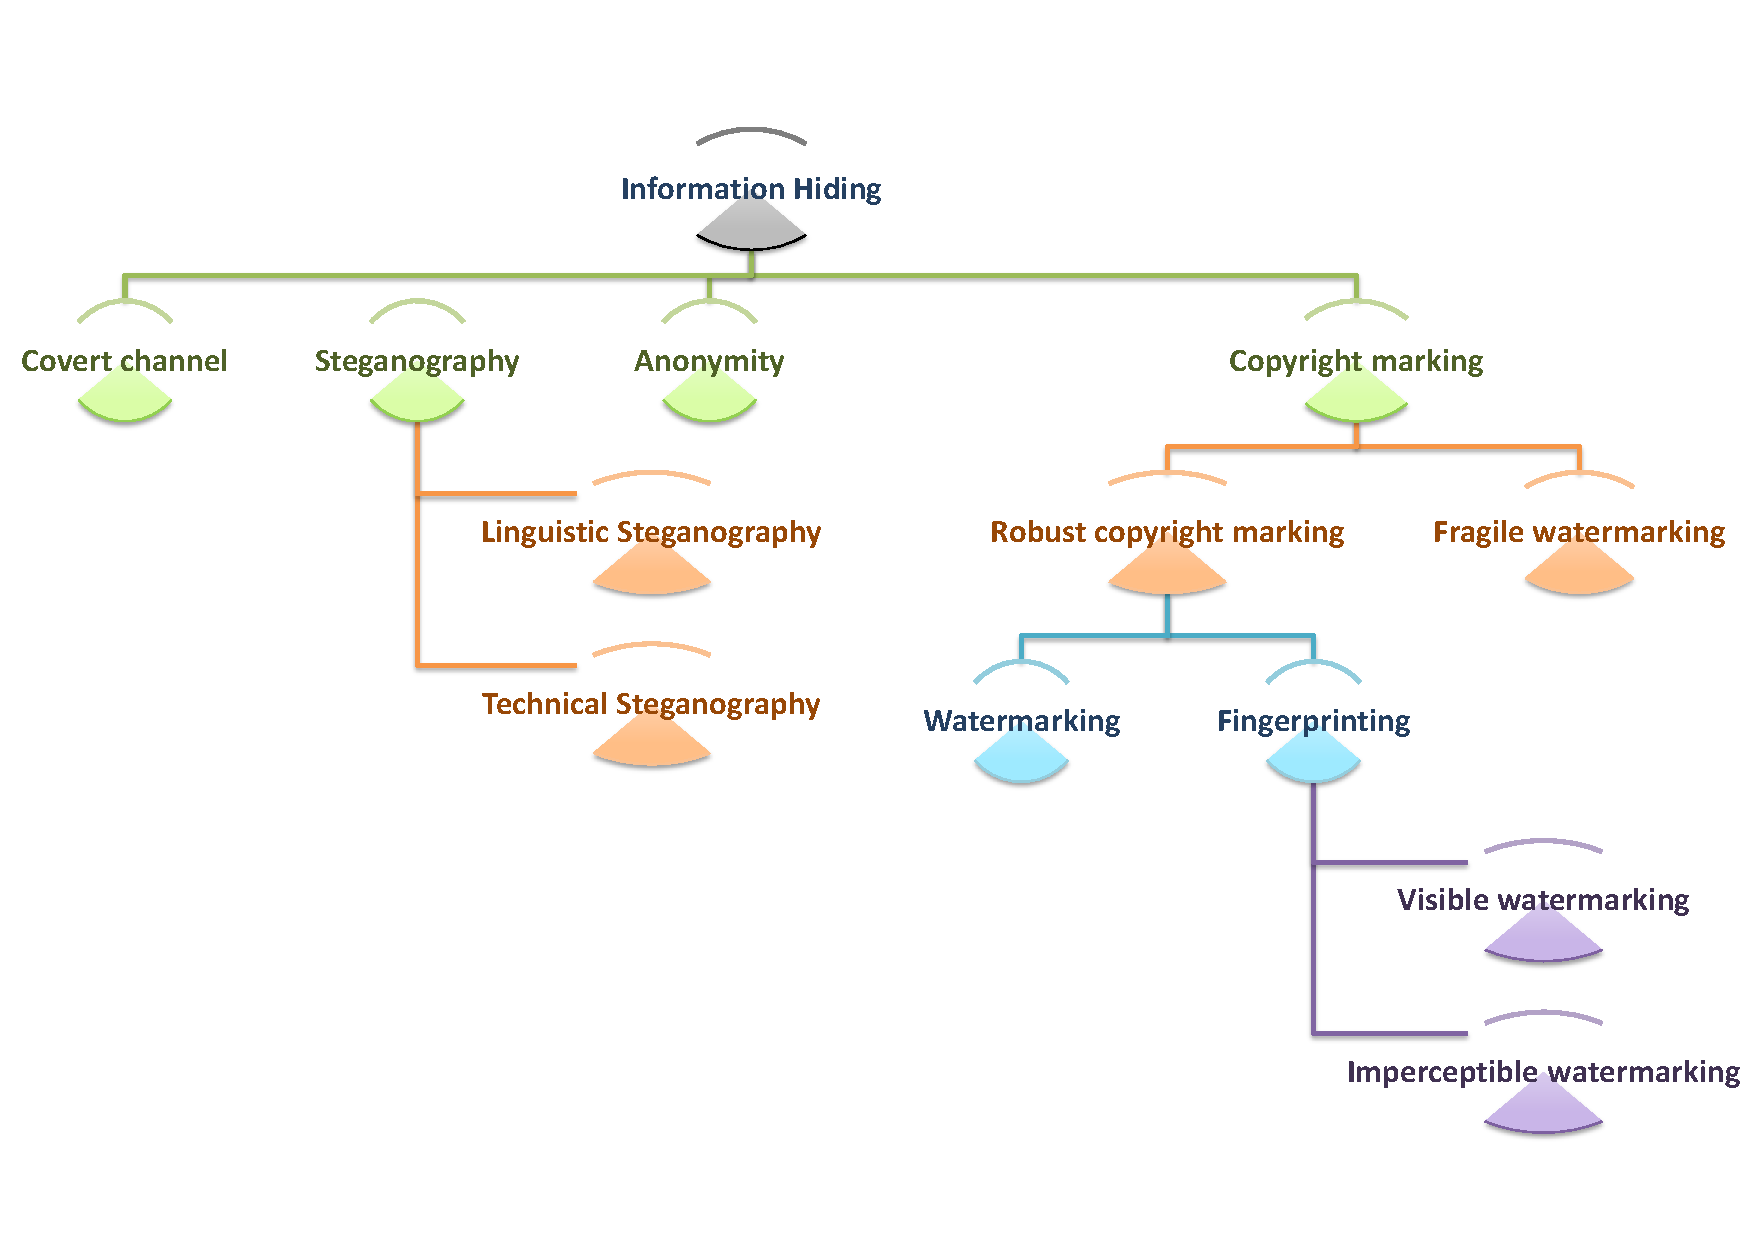
\includegraphics[width=.9\textwidth ,height=.65\textwidth]{Pic/InformationHidingHierarch}
\caption{زیرشاخه‌های علم نهان‌سازی اطلاعات}
\label{InformationHidingHierarch}
\end{figure}

نهان‌سازی به مانند رمزنگاری علمی است چالش برانگیز؛ چراکه در نقطه مقابل نهان‌ساز، فرد یا افرادی وجود دارند، که می‌خواهند کار نهان‌ساز را با شکست مواجه کنند. در این پایان‌نامه ما در دو چهره ظاهر می‌شویم. در چهره اول به عنوان نهان‌ساز به سراغ  می‌رویم، و روشی را در زمینه نشان‌گذاری فایل‌های ویدئویی ارایه می‌دهیم. در چهره بعدی ما دشمن نهان‌ساز می‌شویم. در این چهره به سراغ   ‎\glspl{AggregateFunction}‎  رفته و سعی در کشف پیامی می‌کنیم، که نهان‌نگار آن را در یک سیگنال تصویر پنهان نموده است. 

در نشان‌گذاری به سراغ ویدئو رفتیم؛ چراکه اولا به نظر می‌رسد، نشان‌گذاری در سیگنال تصویر به رشد و بالندگی قابل قبولی رسیده باشد، و الان نیکو است که محور ثقل مطالعات بر روی نشان‌گذاری در ویدئو معطوف شود. دوما به نظر می‌رسد نشان‌گذاری در ویدئو کاربرد بیشتری نسبت به نشان‌گذاری در  تصویر داشته باشد. اما در نهان‌نگاری قضیه کاملا بالعکس است. لذا در مجموع محور مطالعات را بر روی نشان‌گذاری در ویدئو و نهان‌کاوی تصویر، قرار دادیم. 


\section{نهان‌نگاری و نهان‌کاوی}
\label{SteganalysisIntro}

اولین کسی که در تاریخ از این واژه استفاده نمود، فردی به نام {\lr{Johannes Trithemius}} که در سال 1499 در کتابی در مورد جادو، از این واژه استفاده نمود. 

\subsection{آشنایی با چند مفهوم}
برای طی ادامه مسیر لازم است که با برخی مفاهیم موجود در علم ....

\begin{dingautolist}{182}
\item
آیا پیامی‌در سیگنال پنهان شده است یا نه؟
\item
بدست آوردن اطلاعات جانبی از پیام، همچون طول پیامی که پنهان شده است؟
\item
بدست آوردن اصل پیام پنهان شده.
\end{dingautolist}
مهم ترین وظیفه یک نهان‌کاو تشخیص.
\begin{description}
\item[سیگنال پوشش:]\index{سیگنال پوش}
\inpdic{سیگنال پوشش}{Cover Signal}
، سیگنالی است که قصد داریم، در آن پیامی پنهان کنیم. این سیگنال می‌تواند یک تصویر، ویدئو و ... باشد. 
\item[خطای نوع اول:]\index{خطای نوع اول}
خطای نوع اول که آن را با نام {\lr{False Positive}} نیز می‌شناسیم، بدین معنی است که فرستنده پیامی پنهان نکرده باشد، ولی نهان‌کاو به اشتباه بگوید که پیامی در سیگنال پنهان شده است. 
\item[خطای نوع دوم:]\index{خطای نوع دوم}
خطای نوع دوم که آن را با نام {\lr{True Negative}} نیز می‌شناسیم، بدین معنی است که فرستنده پیامی در سیگنال پنهان کرده باشد،
\end{description}


آوردن یک جدول:
\begin{table}
\renewcommand{\arraystretch}{1.35}
\caption{نتایج حمله فشرده سازی \lr{MPEG-4}}
\centering
\begin{tabular}{|c||c|c|c|c|}
\hline
\tablefont{نرخ بیت}&
\tablefont{$1506kbps$}&\tablefont{$1775kbps$}&\tablefont{$1981kbps$}&\tablefont{$2378kbps$}\\\hline
\tablefont{درصد خطا}&\tablefont{$6.05$}&\tablefont{$1.76$}&\tablefont{$0.19$}&\tablefont{$0.58$}\\\hline
\end{tabular}
\label{mpegAttackTable}
\end{table}


\begin{table}
\caption{نتایج حمله بهره}
\centering
\begin{tabular}{|c||c|c|c|c|c|c|}
\hline
\tablefont{ویدئو}&\tablefont{$.1$}&\tablefont{$.3$}&\tablefont{$.5$}&\tablefont{$1.3$}&\tablefont{$1.5$}&\tablefont{$1.7$}\\\hline
\tablefont{foreman}&\tablefont{$0$}&\tablefont{$0$}&\tablefont{$0$}&\tablefont{$2.18$}&\tablefont{$3.24$}&\tablefont{$4.96$}\\\hline
\tablefont{claire}&\tablefont{$3.32$}&\tablefont{$0$}&\tablefont{$0$}&\tablefont{$1.05$}&\tablefont{$0.74$}&\tablefont{$1.32$}\\\hline
\tablefont{hall monitor}&\tablefont{$0$}&\tablefont{$0$}&\tablefont{$0$}&\tablefont{$0$}&\tablefont{$2.03$}&\tablefont{$5.39$}\\\hline
\tablefont{momdaughter}&\tablefont{$0$}&\tablefont{$0$}&\tablefont{$0$}&\tablefont{$0$}&\tablefont{$1.25$}&\tablefont{$2.93$}\\\hline
\end{tabular}
\label{gainAttackTable}
\end{table}

\section{تاثیر تغییر ضریب قدرت }
در این شبیه سازی طول قالب سه بعدی را برابر با $16 \times 16 \times 16$ است. مقدار $\alpha $ را از $1.001$ تا $1.039$ تغییر می‌دهیم. حمله  نویز سفید با انحراف استاندارد 20 را در کانال اعمال می‌کنیم. نتایج برای پنج فایل ویدئویی به صورت زیر است. در این حالت 256 بیت در هر سیگنال پنهان شده است. 












\chapter{وارد کردن فهرست اختصارات}
در این استایل برای تولید فهرست اختصارات از بسته {\lr{glossaries}} استفاده کنید. مراحل تولید فهرست اختصارات بسیار ساده و راحت است. این مراحل به شرح زیر می باشد. 
\begin{itemize}
\arcm
در فایل  ‎\lr{abbr}‎ که در پوشه ‎\lr{Chapters}‎ قرار دارد اختصارات مورد نظر خود را تعریف کنید. برای مثال:
\begin{latin}
\verb+ \newacronym{PSNR}{PSNR}{Peak Signal to Noise Ratio}+
\end{latin}

عنصر اول تعریف فوق، برچسب اختصار، مورد دومی خود اختصار و سومی باز شده آن است. 
\arcm
در هر جای متن که تمایل دارید با دستور  ‎\lr{gls}‎‌و برچسب کلمه اختصار مورد نظر آن را وارد کنید. مثلا:
\verb+\gls{PSNR}+
در این صورت هر جا که این دستور را بنویسید، کلمه ‎\lr{PSNR}‎‌ قرار داده می‌شود. در اولین مکانی که این کلمه را بکار برده‌اید، پاورقی می خورد و به صورت اتوماتیک این کلمه به فهرست اختصارات اضافه می‌شود.
\arcm
در انتهای نیز دنباله زیر را برای تولید فهرست اختصارات انجام دهید:
\begin{LTR}
\begin{itemize}
\tree
\verb+ xelatex -interaction=nonstopmode -synctex=-1 %.tex+
\tree
\verb+ xindy -M %.xdy -t %.nlg -o %.not %.ntn +
\tree
\verb+ xelatex -interaction=nonstopmode -synctex=-1 %.tex+
\tree
\verb+ xelatex -interaction=nonstopmode -synctex=-1 %.tex+
\end{itemize}
\end{LTR}
\end{itemize}
دستور 
\begin{LTR}
\verb+ xelatex -interaction=nonstopmode -synctex=-1 %.tex+
\end{LTR}

همانی است که با   ‎\lr{QuickBuild}‎ زدن اجرا می‌شود. دستور دومی را باید اضافه کنید. برای این کار مثلا برای مثال برای ‎\lr{TexStudio}‎، به منوی ‎\lr{option}‎ و سپس منوی ‎\lr{Configure Texstudio}‎ بروید. در قسمت ‎\lr{Build}‎ و در بخش ‎\lr{User Command}‎ این دستور را اضافه کنید. شکل زیر را مشاهده کنید. 
\begin{figure}[H]
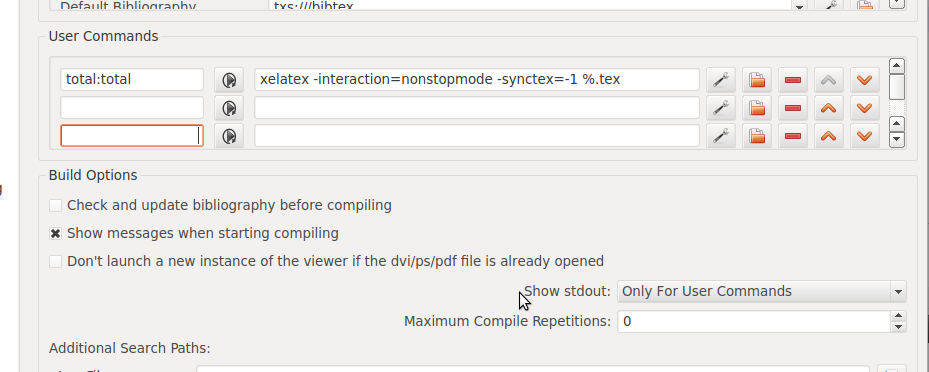
\includegraphics[width=0.9\linewidth]{../Pic/a}
\end{figure}


\chapter{وارد کردن واژه‌نامه}

در ابتدا بسته {\lr{glossaries}} را با {\lr{option}}، {\lr{Xindy}} فراخوانی کنید. در مرحله بعد دو استایل برای واژه نامه ها با دستور {\lr{newglossarystyle}} تعریف نموده ایم. یکی برای واژه نامه فارسی به انگلیسی یکی هم برای انگلیسی به فارسی. 

در مرحله سوم دو نوع واژه نامه بادستور {\lr{newglossary}} تعریف می کنیم. دقت کنید با این کار ۵ فایل با پسوند {\lr{blo,glo,gls,glo,glg}} تولید می شود.

در فایل ‎\lr{Words}‎ در پوشه ‎\lr{Chapters}‎، شما می‌توانید واژه ها خود را تعریف کنید. اگر فایل مورد نظر را مشاهده کنید، می بینید که مثلا من یک کلمه به نام ‎\lr{Absorption}‎ به معنی جذب تعریف کرده‌ام. اکنون کافی است که شما هرجای متن که می خواهید کلمه جذب ظاهر شود بنویسید (به این قسمت در فایل ‎\lr{Tex}‎مراجعه کنید. )

این یک مثال از \glspl{Absorption} است.

این مورد نیز به مانند اختصارات، به صورت خودکار اولین جا پاورقی می خورد و در دو واژه نامه وارد و مرتب می شود، 


مهم ترین مرحله کامپایل برنامه است که باید به صورت دنباله زیر باشد:
\begin{itemize}
\begin{LTRitems}
\hand
\verb+ xelatex -interaction=nonstopmode -synctex=-1 %.tex+
\hand
\verb+ xindy -L persian-variant1 -C utf8 -I xindy -M %.xdy -t %.glg -o %.gls %.glo +
\hand
\verb+ xindy -L persian-variant1 -C utf8 -I xindy -M %.xdy -t %.blg -o %.bls %.blo +
\hand
\verb+ xelatex -interaction=nonstopmode -synctex=-1 %.tex+
\end{LTRitems}
\end{itemize}
به مانند اختصارات این دو دستور را در ‎\lr{Texstudio}‎‌خود معرفی کنید. 

مثال‌هایی دیگر، به فایل ‎\lr{Tex}‎ نگاه کنید. 
\glspl{AcceptableCell}

\glspl{Accessibility}

\glspl{AccessDomain}









\chapter{وارد کردن مراجع}
برای وارد کردن مراجع در پایان‌نامه بهترین روش استفاده از \lr{bibtex} است. 


برای مثال مرجع {\cite{Mackey2005_Effects}} در مورد شبکه .... . و این هم مرجع دوم {\cite{Kappler2009}} 

و سپس مرجع سوم {\cite{Kappler2009}}

برای آوردن مراجع باید مراحل زیر را انجام دهید.
\begin{itemize}
\begin{LTRitems}
\item
\verb+ xelatex -interaction=nonstopmode -synctex=-1 %.tex+
\item
\verb+ bibtex  % +
\item
\verb+ xelatex -interaction=nonstopmode -synctex=-1 %.tex+
\item
\verb+ xelatex -interaction=nonstopmode -synctex=-1 %.tex+
\end{LTRitems}
\end{itemize}
اگر از ویرایشگر {\lr{Texmaker}} استفاده می‌کنید، دستور اولی، سومی و چهارمی همان {\lr{Quick Build}} است. یعنی اگر دکمه {\lr{Quick Build}} را بزنید، انگار دستور مورد اشاره را اجرا کرده اید. در مورد دستور دوم، در {\lr{Texmaker}} همان دستور {\lr{bibtex}} است. در اکثر ویرایشگرها چنین چیزی وجود دارد.  

% انواع دیگر استایل ها در راهنمای persian-bib آمده است. 





\chapter{وارد کردن کد در متن}
برای وارد کردن کدهای برنامه نویسی خود در محیط لاتک، بسته \lr{listings} یکی از بهترین بسته های موجود است. برای استفاده از این بسته فقط به نکات زیر دقت کنید:
\begin{itemize}
\hand
در شروع امر بسته \lr{listings} را  با دستور \lr{usepackage} فراخوانی کنید. دقت کنید که این بسته را با بسته \lr{listing} اشتباه نکنید.
\hand
در مرحله بعدی می توانید توسط دستور \lr{lstset} هرجایی از متن که خواستید تنظیمات این بسته را تغییر دهید. 
\hand
در هنگام استفاده از این بسته فقط دقت داشته باشید که محیط آن باید بین محیط \lr{latin}‌قرار گیرد. 
\hand
دو راهنمایی خوب برای این بسته یکی سایت \lr{http://en.wikibooks.org/wiki/LaTeX/Packages/Listings}‌ ودیگری راهنمای این بسته است. 
\hand
برای فهم بهتر این مثال بهتر است که مثال را از فایل \lr{tex} دنبال کنید نه از فایل \lr{pdf} چراکه بسیاری از توضیحات به صورت \lr{comment} در فایل \lr{tex} داده شده است. 
\end{itemize}


مثالی از نوشتن کد مطلب درون یک نوشتار:

\begin{latin}
\lstinputlisting[language=Matlab]{Code/code3.m}
\end{latin}

در این مثال یک کد \lr{MATLAB} دیگر وارد می کنیم، با این تفاوت که می خواهیم یکسری از کلمات کلیدی را مشخص کنیم که لاتک آن ها را با رنگی به خصوصی نشان دهد. 
\begin{latin}
\lstset{emph={binornd},emphstyle=\color{Magenta}}
\lstinputlisting[language=Matlab, morekeywords={ksdensity}]{Code/prog3.m}
\end{latin}

مثالی دیگر از نوشتن کد مطلب در یک نوشتار. فقط در این حالت می خواهیم برخی از تنظیمات پیش فرض را که قبل از شروع نوشتار تعیین کرده ایم، تغییر دهیم. 
\begin{latin}
\lstinputlisting[numbers=right,language=Matlab, framexleftmargin=5mm, frame=shadowbox,rulesepcolor=\color{Yellow}]{Code/code4.m}
\end{latin}

مثالی از نوشتن یک کد {\lr{JAVA}} درون یک نوشتار:

\definecolor{codeColor}{rgb}{0.9,0.9,0.9}
\begin{latin}
\lstset{emph={pMax,pMin,transP,waitingUser,waitQueue},emphstyle=\color{red},backgroundcolor=\color{codeColor},lineskip=.2cm}
\lstinputlisting[language=Java]{Code/threadQueue.java}
\end{latin}

در ضمن شما می توانید حتی در خود همین نوشتار اصلی خود کد مورد نظرتان را بنویسید. 
\begin{latin}
\lstset{frameshape={RYRYNYYYY}{yny}{yny}{RYRYNYYYY}}
\begin{lstlisting}
for i:=maxint to 0 do
begin
{ do nothing }
end;
\end{lstlisting}
\end{latin}




%%%%%%%%%%%%
% آوردن مراجع در انتهای گزارش با فرمت IEEE 
% فرمت مراجع می تواند برای ACM و ... نیز باشد. برای این کار کافی است تنها 
%پارامتر style را باید تغییر دهید. 
\baselineskip=.65cm

% مراجع همگی در یک فایل bibtex با پسوند .bib  وجود دارد، که می بایست در پوشه اصلی گزارش قرار داده شود.
% نام این فایل می بایست library باشد. در غیر این صورت باید نام فایل bib را در خط زیر تغییر دهید. 
%\renewcommand{\bibname}{مراجع}
\clearpage
\phantomsection
%\addcontentsline{toc}{chapter}{کتاب نامه}
\bibliographystyle{plain-fa}%{persia}
\bibliography{library}




%%%%%%%%%%
\baselineskip=.75cm
\glossarystyle{mylist1}
\clearpage
\phantomsection
\def\glossaryname{واژه نامه فارسی به انگلیسی}
\addcontentsline{toc}{chapter}{\glossaryname}
\printglossary[title={ \glossaryname}]

% قرار دادن واژه نامه انگلیسی به فارسی

\begin{LTR}
\def\glossaryname{\rl{واژه نامه انگلیسی به فارسی}}
%\addcontentsline{toc}{chapter}{\glossaryname}
\begin{LTR}
\printglossary[type={mylist1},title={\begin{center} \glossaryname \end{center}}]
\end{LTR}
\end{LTR}



%%%%%%%%%%
% قرار دادن نمایه کلمات به عنوان آخرین قسمت گزارش
\baselineskip=.75cm
\clearpage
\phantomsection
\addcontentsline{toc}{chapter}{نمایه}
\printindex



\thispagestyle{empty} %prevents tex from numbering of this page
\begin{latin} % xepersian enviorment

\centerline{\textbf{\large{Abstract}}}
\vskip 1cm

Steganography is the art and science of writing hidden messages in such a way that no one, apart from the sender and intended recipient, suspects the existence of the message, a form of security through obscurity.

In this thesis, we focus on  entropic issue of multimedia signal in the two branches of Information hiding namely Steganography and  Watermarking. How to choose the block and noise estimation in the watermarking, and analysis of the singular values decomposition in steganography are examples of using entopic issue which we use in our thesis. 

The two new designs for video signals AVI are presented in Watermarking. For the both proposed method ,first AVI video signal will be divided into several part and each part  will be divided into several three-dimensional block. 3D block with maximum entropy is chosen, then the watermarks are embedded in the low-frequency wavelet transform coefficients of 3D chosen block. Inthe first proposed method, the sender must send some statistical data of AVI signal through a secure channel to the receiver. The receiver uses these information to detect Watermark using Maximum Likelihood scheme. Inthe second proposed method, the receiver do not need to statistical information of signal. We evaluate  the performance of the proposed method with theory and simulation.

In the Steganalysis, we suppose  LSB as steganography method. We focus on singular value decomposition which shows the entropy of the our image signal. If a message is added to the signal, the entropy of the signal increase. Amount of entropy related to the main content of the message signal. We try to estimate the singular values ​​to detect which signal is a  clean or stego. We can also use this method as approximation of  Steganography rate. Support Vector Machine and the noise estimation of the image signal are two tools in order to achieve a better and more accurate steganalysis. To better evaluate the proposed method, a comprehensive database of images is used in the simulations.

Keywords: Steganography, Steganalysis, Watermarking, Blind Watermarking, semi blind Watermarking, LSB Method.

\end{latin}

\clearpage
\input{Chapters/cover_en}



% % % % % % % % % % % % % % % % % % % % % % % % % % 

% وارد کردن مراجع، به عنوان آرگومان ورودی کافی است که نام فایل با پسوند .bib را بدهید. 
\bibliography{library}
% برای تولید هر دو واژه‌نامه کافی است دستور زیر را وارد کنید. 
\printglossary
% برای تولید نمایه کافی است که دستور زیر استفاده کنید، و درون متن نیز کلمه‌ای را که می‌خواهد در نمایه بیاید با دستور \index{} مشخص کنید. 
\printindex

%\thispagestyle{empty} %prevents tex from numbering of this page
\begin{latin} % xepersian enviorment

\centerline{\textbf{\large{Abstract}}}
\vskip 1cm

Steganography is the art and science of writing hidden messages in such a way that no one, apart from the sender and intended recipient, suspects the existence of the message, a form of security through obscurity.

In this thesis, we focus on  entropic issue of multimedia signal in the two branches of Information hiding namely Steganography and  Watermarking. How to choose the block and noise estimation in the watermarking, and analysis of the singular values decomposition in steganography are examples of using entopic issue which we use in our thesis. 

The two new designs for video signals AVI are presented in Watermarking. For the both proposed method ,first AVI video signal will be divided into several part and each part  will be divided into several three-dimensional block. 3D block with maximum entropy is chosen, then the watermarks are embedded in the low-frequency wavelet transform coefficients of 3D chosen block. Inthe first proposed method, the sender must send some statistical data of AVI signal through a secure channel to the receiver. The receiver uses these information to detect Watermark using Maximum Likelihood scheme. Inthe second proposed method, the receiver do not need to statistical information of signal. We evaluate  the performance of the proposed method with theory and simulation.

In the Steganalysis, we suppose  LSB as steganography method. We focus on singular value decomposition which shows the entropy of the our image signal. If a message is added to the signal, the entropy of the signal increase. Amount of entropy related to the main content of the message signal. We try to estimate the singular values ​​to detect which signal is a  clean or stego. We can also use this method as approximation of  Steganography rate. Support Vector Machine and the noise estimation of the image signal are two tools in order to achieve a better and more accurate steganalysis. To better evaluate the proposed method, a comprehensive database of images is used in the simulations.

Keywords: Steganography, Steganalysis, Watermarking, Blind Watermarking, semi blind Watermarking, LSB Method.

\end{latin}


\englishcover

\end{document}
